\PassOptionsToPackage{unicode=true}{hyperref} % options for packages loaded elsewhere
\PassOptionsToPackage{hyphens}{url}
%
\documentclass[]{book}
\usepackage{lmodern}
\usepackage{amssymb,amsmath}
\usepackage{ifxetex,ifluatex}
\usepackage{fixltx2e} % provides \textsubscript
\ifnum 0\ifxetex 1\fi\ifluatex 1\fi=0 % if pdftex
  \usepackage[T1]{fontenc}
  \usepackage[utf8]{inputenc}
  \usepackage{textcomp} % provides euro and other symbols
\else % if luatex or xelatex
  \usepackage{unicode-math}
  \defaultfontfeatures{Ligatures=TeX,Scale=MatchLowercase}
\fi
% use upquote if available, for straight quotes in verbatim environments
\IfFileExists{upquote.sty}{\usepackage{upquote}}{}
% use microtype if available
\IfFileExists{microtype.sty}{%
\usepackage[]{microtype}
\UseMicrotypeSet[protrusion]{basicmath} % disable protrusion for tt fonts
}{}
\IfFileExists{parskip.sty}{%
\usepackage{parskip}
}{% else
\setlength{\parindent}{0pt}
\setlength{\parskip}{6pt plus 2pt minus 1pt}
}
\usepackage{hyperref}
\hypersetup{
            pdftitle={Term project draft},
            pdfauthor={Kipling Klimas},
            pdfborder={0 0 0},
            breaklinks=true}
\urlstyle{same}  % don't use monospace font for urls
\usepackage{color}
\usepackage{fancyvrb}
\newcommand{\VerbBar}{|}
\newcommand{\VERB}{\Verb[commandchars=\\\{\}]}
\DefineVerbatimEnvironment{Highlighting}{Verbatim}{commandchars=\\\{\}}
% Add ',fontsize=\small' for more characters per line
\usepackage{framed}
\definecolor{shadecolor}{RGB}{248,248,248}
\newenvironment{Shaded}{\begin{snugshade}}{\end{snugshade}}
\newcommand{\AlertTok}[1]{\textcolor[rgb]{0.94,0.16,0.16}{#1}}
\newcommand{\AnnotationTok}[1]{\textcolor[rgb]{0.56,0.35,0.01}{\textbf{\textit{#1}}}}
\newcommand{\AttributeTok}[1]{\textcolor[rgb]{0.77,0.63,0.00}{#1}}
\newcommand{\BaseNTok}[1]{\textcolor[rgb]{0.00,0.00,0.81}{#1}}
\newcommand{\BuiltInTok}[1]{#1}
\newcommand{\CharTok}[1]{\textcolor[rgb]{0.31,0.60,0.02}{#1}}
\newcommand{\CommentTok}[1]{\textcolor[rgb]{0.56,0.35,0.01}{\textit{#1}}}
\newcommand{\CommentVarTok}[1]{\textcolor[rgb]{0.56,0.35,0.01}{\textbf{\textit{#1}}}}
\newcommand{\ConstantTok}[1]{\textcolor[rgb]{0.00,0.00,0.00}{#1}}
\newcommand{\ControlFlowTok}[1]{\textcolor[rgb]{0.13,0.29,0.53}{\textbf{#1}}}
\newcommand{\DataTypeTok}[1]{\textcolor[rgb]{0.13,0.29,0.53}{#1}}
\newcommand{\DecValTok}[1]{\textcolor[rgb]{0.00,0.00,0.81}{#1}}
\newcommand{\DocumentationTok}[1]{\textcolor[rgb]{0.56,0.35,0.01}{\textbf{\textit{#1}}}}
\newcommand{\ErrorTok}[1]{\textcolor[rgb]{0.64,0.00,0.00}{\textbf{#1}}}
\newcommand{\ExtensionTok}[1]{#1}
\newcommand{\FloatTok}[1]{\textcolor[rgb]{0.00,0.00,0.81}{#1}}
\newcommand{\FunctionTok}[1]{\textcolor[rgb]{0.00,0.00,0.00}{#1}}
\newcommand{\ImportTok}[1]{#1}
\newcommand{\InformationTok}[1]{\textcolor[rgb]{0.56,0.35,0.01}{\textbf{\textit{#1}}}}
\newcommand{\KeywordTok}[1]{\textcolor[rgb]{0.13,0.29,0.53}{\textbf{#1}}}
\newcommand{\NormalTok}[1]{#1}
\newcommand{\OperatorTok}[1]{\textcolor[rgb]{0.81,0.36,0.00}{\textbf{#1}}}
\newcommand{\OtherTok}[1]{\textcolor[rgb]{0.56,0.35,0.01}{#1}}
\newcommand{\PreprocessorTok}[1]{\textcolor[rgb]{0.56,0.35,0.01}{\textit{#1}}}
\newcommand{\RegionMarkerTok}[1]{#1}
\newcommand{\SpecialCharTok}[1]{\textcolor[rgb]{0.00,0.00,0.00}{#1}}
\newcommand{\SpecialStringTok}[1]{\textcolor[rgb]{0.31,0.60,0.02}{#1}}
\newcommand{\StringTok}[1]{\textcolor[rgb]{0.31,0.60,0.02}{#1}}
\newcommand{\VariableTok}[1]{\textcolor[rgb]{0.00,0.00,0.00}{#1}}
\newcommand{\VerbatimStringTok}[1]{\textcolor[rgb]{0.31,0.60,0.02}{#1}}
\newcommand{\WarningTok}[1]{\textcolor[rgb]{0.56,0.35,0.01}{\textbf{\textit{#1}}}}
\usepackage{longtable,booktabs}
% Fix footnotes in tables (requires footnote package)
\IfFileExists{footnote.sty}{\usepackage{footnote}\makesavenoteenv{longtable}}{}
\usepackage{graphicx,grffile}
\makeatletter
\def\maxwidth{\ifdim\Gin@nat@width>\linewidth\linewidth\else\Gin@nat@width\fi}
\def\maxheight{\ifdim\Gin@nat@height>\textheight\textheight\else\Gin@nat@height\fi}
\makeatother
% Scale images if necessary, so that they will not overflow the page
% margins by default, and it is still possible to overwrite the defaults
% using explicit options in \includegraphics[width, height, ...]{}
\setkeys{Gin}{width=\maxwidth,height=\maxheight,keepaspectratio}
\setlength{\emergencystretch}{3em}  % prevent overfull lines
\providecommand{\tightlist}{%
  \setlength{\itemsep}{0pt}\setlength{\parskip}{0pt}}
\setcounter{secnumdepth}{5}
% Redefines (sub)paragraphs to behave more like sections
\ifx\paragraph\undefined\else
\let\oldparagraph\paragraph
\renewcommand{\paragraph}[1]{\oldparagraph{#1}\mbox{}}
\fi
\ifx\subparagraph\undefined\else
\let\oldsubparagraph\subparagraph
\renewcommand{\subparagraph}[1]{\oldsubparagraph{#1}\mbox{}}
\fi

% set default figure placement to htbp
\makeatletter
\def\fps@figure{htbp}
\makeatother

\usepackage{booktabs}
\usepackage[]{natbib}
\bibliographystyle{apalike}

\title{Term project draft}
\author{Kipling Klimas}
\date{2021-03-21}

\begin{document}
\maketitle

{
\setcounter{tocdepth}{1}
\tableofcontents
}
\hypertarget{introduction}{%
\chapter{Introduction}\label{introduction}}

Wildfires can have significant impacts on both ecosystems and human assets in forested environments. In the fire-prone mixed conifer/aspen forests of the Intermountain West (IW) fuel reduction treatments including stand thinning, mastication, aspen promotion and prescribed fire are implemented to reduce the risk, incidence and/or extent of destructive, high severity wildfire. Due to the high value of forested resources in the IW and the risk of post-fire sediment transport or debris flows downstream from burned areas, fuel reduction treatments are important landscape-scale tools that forest managers use to protect forest assets. However, the complex and pyrophytic nature of IW forests, along environmental and societal constraints, lends to barriers against spatially targeted implementation of fuel reduction treatments in high-value forested watersheds (Larson \& Churchill, 2012).

Modeling the effect of fuel reduction treatments on fire behavior in fire-prone forests of the western United States has shown that targeted fuel reduction treatments are more effective at altering fire behavior (i.e.~rate of spread, flame length) than randomly or indiscriminately applied treatments (Kim et al., 2009; Minas et al., 2014; Prichard et al., 2020). The spatial distribution of treatments must then follow a prioritization hierarchy, such as concentrated, dispersed or regularly arranged treated areas within a forest (Kim et al., 2009), but the economic trade-off and efficacy of treatment distribution warrants greater examination in IW forests, where fuel treatments are applied to reduce the risk of high severity wildfire (Barros et al., 2019). By altering fire behavior through landscape-scale treatments, forest managers hope to reduce the extent of high-severity burned areas and mitigate downstream consequences of high-severity wildfire, such as the development of debris flows which can have negative impacts on high value assets such as reservoirs or fish habitat.

\hypertarget{data}{%
\chapter{Data description and database structure}\label{data}}

Forest strcuture and fuels data are needed to model fire behavior and predict burn severity spatially.

\begin{center}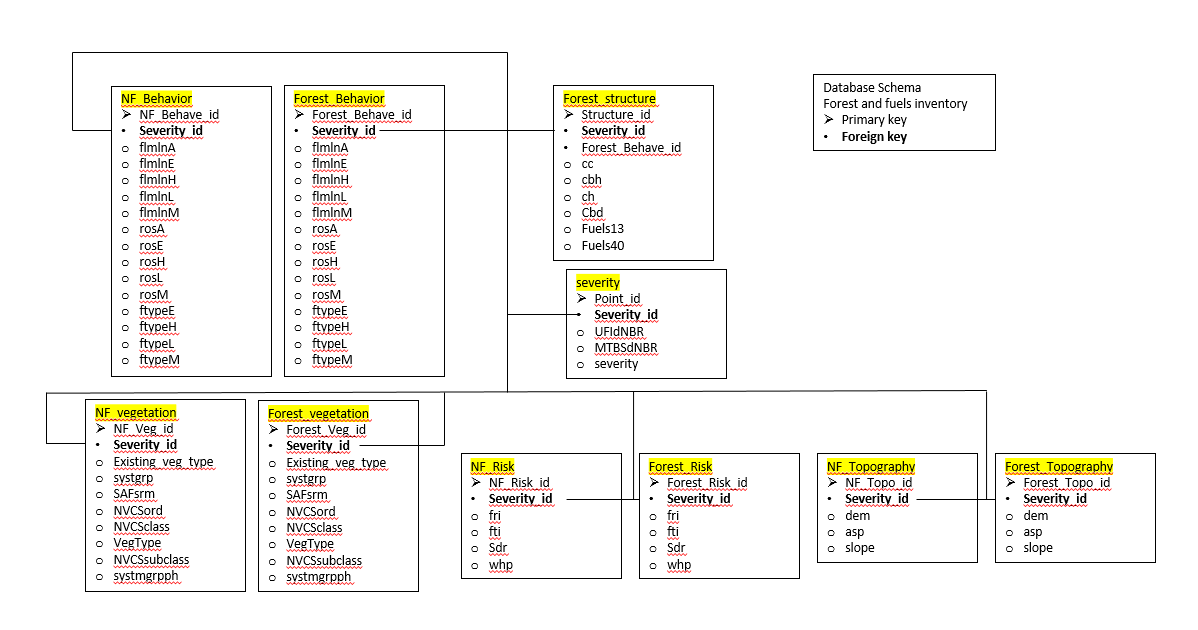
\includegraphics{db_structure} \end{center}

Figure 1: databse structure for forest and fuels inventory.

This database structure is compatible with tree and stand level forest simulation software such as the Forest Vegetation Simulator (FVS) which can be used to model forest structure over time. An advantage of this approach and structure is these data allow detailed simulation of mortality during fire.

Tree level data are related to plot polygons that allow for stand-level simulation. Fuels data is required for modeled fire behavior, such as flame length, rate or spread or fire type (surface, passive or active).

Whether or not these tables become populated remains to be seen- a disadvantage of this approach is that fuel reduction treatments are not readily applied to the landscape in question. It is also only useable for fire behavior modeling as an ArcMap toolbar extension.

\hypertarget{creation}{%
\chapter{Database creation}\label{creation}}

Start

Install and open packages \texttt{RSQLite}

\begin{Shaded}
\begin{Highlighting}[]
\KeywordTok{install.packages}\NormalTok{(}\StringTok{"RSQLite"}\NormalTok{)}
\KeywordTok{library}\NormalTok{(RSQLite)}
\end{Highlighting}
\end{Shaded}

Establish database connection

Connecting to the term\_project database

\begin{Shaded}
\begin{Highlighting}[]
\NormalTok{term_project <-}\StringTok{ }\KeywordTok{dbConnect}\NormalTok{(}\DataTypeTok{drv =}\NormalTok{ RSQLite}\OperatorTok{::}\KeywordTok{SQLite}\NormalTok{(),}
                        \StringTok{"/Users/kiplingklimas/Box/Lab_Group/Kipling/Classes/WILD6900_EcoRepSci/databases/term_project.db"}\NormalTok{)}
\end{Highlighting}
\end{Shaded}

Create trees table
Term project database creation based on structure in figure 1

\begin{Shaded}
\begin{Highlighting}[]
\KeywordTok{dbExecute}\NormalTok{(term_project, }\StringTok{"CREATE TABLE trees(}
\StringTok{tree_id integer PRIMARY KEY AUTOINCREMENT,}
\StringTok{tree_number varchar(5),}
\StringTok{plot_id float,}
\StringTok{stand_id float,}
\StringTok{tree_sp varchar(4),}
\StringTok{dbh_cm float,}
\StringTok{height_cm float, }
\StringTok{cbh_cm float,}
\StringTok{FOREIGN KEY(plot_id) REFERENCES plots(plot_id)}
\StringTok{FOREIGN KEY(stand_id) REFERENCES stands(stand_id)}
\StringTok{);"}\NormalTok{)}
\end{Highlighting}
\end{Shaded}

Create stands table

\begin{Shaded}
\begin{Highlighting}[]
\KeywordTok{dbExecute}\NormalTok{(term_project, }\StringTok{"CREATE TABLE stands(}
\StringTok{stand_id integer PRIMARY KEY AUTOINCREMENT,}
\StringTok{stand_number varchar(5),}
\StringTok{plot_id float,}
\StringTok{ba_m_ha float,}
\StringTok{cbd_kg_m3 float,}
\StringTok{tpa float,}
\StringTok{cc_percent float,}
\StringTok{stand_density float, }
\StringTok{FOREIGN KEY(plot_id) REFERENCES plots(plot_id)}
\StringTok{);"}\NormalTok{)}
\end{Highlighting}
\end{Shaded}

Create fuels table

\begin{Shaded}
\begin{Highlighting}[]
\KeywordTok{dbExecute}\NormalTok{(term_project, }\StringTok{"CREATE TABLE fuels(}
\StringTok{fuel_id integer PRIMARY KEY AUTOINCREMENT,}
\StringTok{stand_id float,}
\StringTok{plot_id float,}
\StringTok{fuel_model varchar(6),}
\StringTok{one_hr float,}
\StringTok{ten_hr float,}
\StringTok{hundred_hr float,}
\StringTok{thousand_hr float,}
\StringTok{coarse_wd float,}
\StringTok{fine_wd float,}
\StringTok{FOREIGN KEY(stand_id) REFERENCES stands(stand_id)}
\StringTok{FOREIGN KEY(plot_id) REFERENCES plots(plot_id)}
\StringTok{);"}\NormalTok{)}
\end{Highlighting}
\end{Shaded}

Create plots table

\begin{Shaded}
\begin{Highlighting}[]
\KeywordTok{dbExecute}\NormalTok{(term_project, }\StringTok{"CREATE TABLE plots(}
\StringTok{plot_id integer PRIMARY KEY AUTOINCREMENT,}
\StringTok{stand_id float,}
\StringTok{fuel_id float,}
\StringTok{plot_number float,}
\StringTok{plot_area_m2 float,}
\StringTok{date text,}
\StringTok{utm_x float,}
\StringTok{utm_y float,}
\StringTok{elevation float,}
\StringTok{slope float,}
\StringTok{aspect varchar(3),}
\StringTok{county text,}
\StringTok{ranger_district text,}
\StringTok{FOREIGN KEY(stand_id) REFERENCES stands(stand_id)}
\StringTok{FOREIGN KEY(fuel_id) REFERENCES fuels(fuel_id)}
\StringTok{);"}\NormalTok{)}
\end{Highlighting}
\end{Shaded}

\bibliography{book.bib,packages.bib}

\end{document}
